\documentclass[pdftex,12pt,letter]{article}
\usepackage[binary-units=true]{siunitx}
\usepackage[margin=0.75in]{geometry}
\usepackage[utf8]{inputenc}
\usepackage[T1]{fontenc}
\usepackage{graphicx}
\usepackage{amsmath}
\usepackage{xspace}
\usepackage{xcolor}
\usepackage[pdftex,pdfpagelabels,bookmarks,hyperindex,hyperfigures]{hyperref}

\newcommand{\fixme}[1]{\textcolor{red}{\textit{Fixme}: \textbf{#1}}}


\author{Brett Viren}
\date{\today}
\title{Single-Phase protoDUNE TPC \\ Detector Element Connectivity\\{\small DUNE DocDB 4064}}
\begin{document}

\maketitle

\begin{abstract}
  \noindent The connectivity of detector elements relevant to TPC wire
  data from the single-phase protoDUNE experiment is described.  It is
  expressed as a directed graph of ordered edges.  Edges map to
  connections between detector elements following minimal and local
  numbering conventions taken from the installation and engineering
  designs for the hardware involved.  Schemes for flattening this
  graph and producing global numbering conventions are proposed.
  Software to produce a instances of connection graphs is described
  and a sample of the diagrams it can generate are included for
  illustration and validation purposes.
\end{abstract}

%\newpage
\tableofcontents
\newpage
\section{Overview}

This document describes a \textit{directed, cyclic graph} representing
the connections between the detector elements (aka parts) of the
single-phase protoDUNE detector related to TPC wire data.  A
\textit{node} in the graph represents a particular detector element
which has importance for analyzing and simulating the detector data.
An \textit{edge} in the graph represents a logical or physical
connection between two types of parts.  An edge which represents a
parent/child relationship carries one or more \textit{attributes}
(typically, sequence indices) which allow a parent's children to be ordered and
to then associate their order with actual connections in the real
detector.  As such, the nodes themselves do not hold attributes that
provide identity.  Rather, nodes are identified by their location in
the graph relative to other nodes.  Some nodes do carry attributes
which represent physical quantities such as their position in space.

In determining the connectivity between nodes, the edges and their
index attributes are chosen to follow engineering and design documents and
drawings.  This allows the graph representation to be independent of
any global numbering convention while still correctly representing the
design.  It also happens to allow representing connectivity which
deviates from design as may arise from mistakes during cabling or with
DAQ configuration.  As such are found and fixed, different graphs may
be constructed to account for and record the changes.

While the edge attributes assert a minimal local numbering convention
they do not preclude more prescriptive or global conventions to be
defined as a function of the resulting graph.  Indeed, multiple useful
conventions must likely emerge from this graph depending on the
context in which the connection information is needed.  For example,
when debugging hardware issues it will be best to have waveform data
associated with a tuple of numbers (APA, WIB, WIB slot, front-end
electronics board, preamp/ADC chip pair, and the chip's ``channel'').
On the other hand, with reconstruction and simulation software it is
important to identify a waveform with a wire segment described by a
different tuple: (APA, face, plane, conductor, segment).  By the
nature of the protoDUNE design, the mapping between these tuples is
not trivial and requires a graph traversal.

So, developing conventions to provide a flat sequence of numbers which
enumerate parts at some more global scale is needed.  For example, it
is expected that numbering the 400, 400 or 480 ``spots'' where a
conductor terminates on wire boards in one of the three planes,
respectively, in an APA face will be a useful intermediate flat
numbering scheme for producing visualizations of waveform samples vs
time to understand activity in the detector (``event displays'').
While the wrapping of the induction conductors will lead to some
ambiguity this will give much more understandable views of the data
than would plotting waveforms ordered by board-chip-channel.

The rest of this section defines the detector elements considered in
the connectivity graph as well as the orientation labels and
coordinate system conventions used.  Next, the types of connection are
described in some detail.  Then, schemes for generating ``flat'' or
global numbering conventions are presented.  Finally, some description
of the software used to generate, visualize and validate the
connection graph is provided.


\subsection{Detector Elements}
\label{sec:parts}

Figure~\ref{fig:schema} shows a \textit{schema graph} which
illustrates the node and edge types that are employed in the full
detector element connectivity graph.  It also indicates labels for
edge attributes which hold sequence indices.  The full connectivity
graph can be understood as an expansion of this schema graph by
iterating over these indices in ranges indicated by the multiplicities
shown the node boxes while constrained by the actual connections
defined by the protoDUNE design.

\begin{figure}[h]
  \centering
  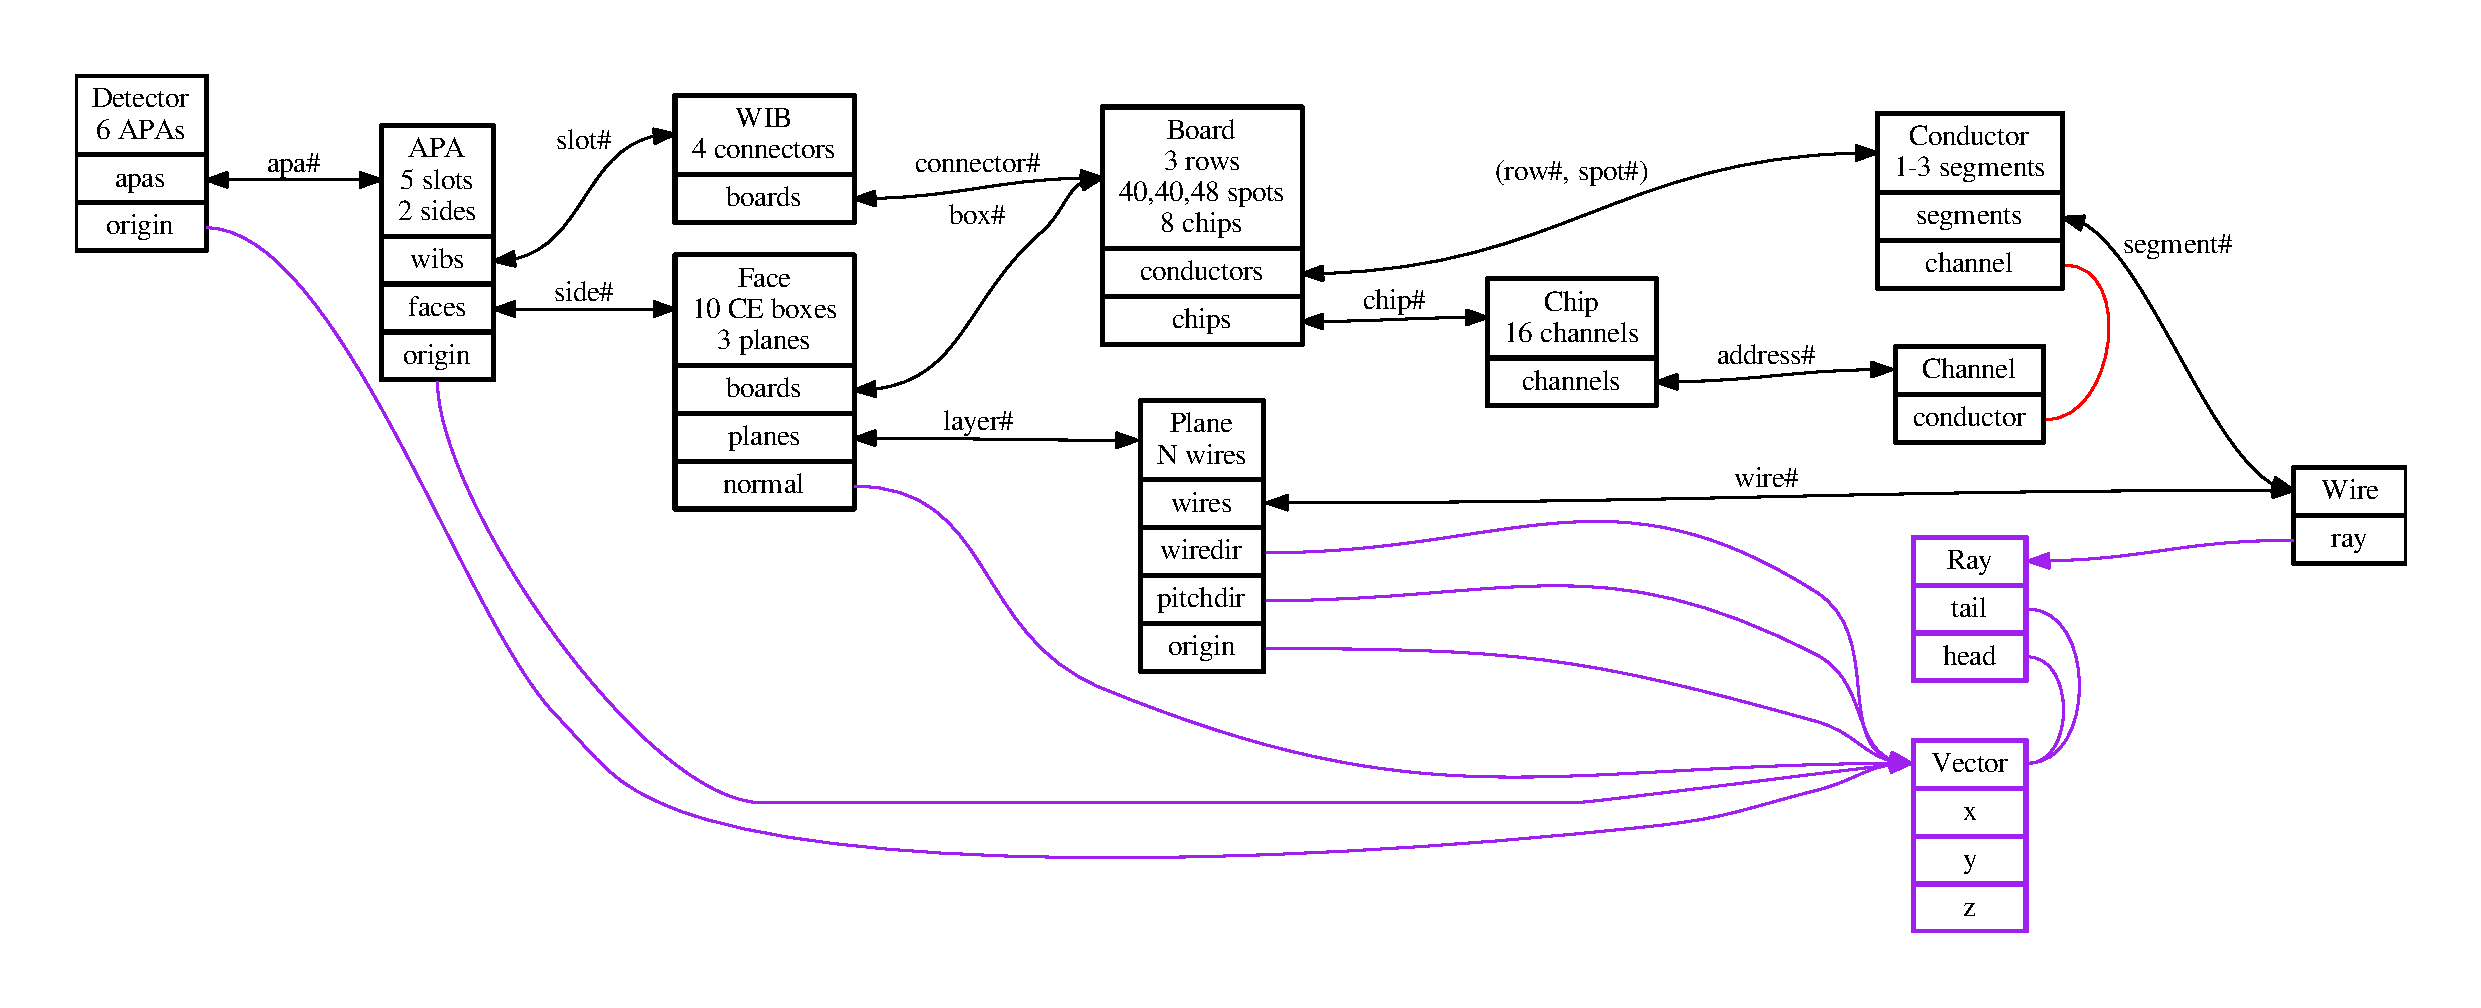
\includegraphics[width=\textwidth]{dots/schema2.pdf}
  \caption[Connectivity schema graph.]{A graph representation of the \textit{schema} which the detector element connectivity graph follows.  Black arrows indicate a parent/children relationship.  The relationship has edge attributes (indices) which allow for ordering and association with physical connectivity.   Purple indicate associated geometry information and red indicate one-to-one relationships. }
  \label{fig:schema}
\end{figure}

\pagebreak

\noindent The nodes in the schema graph and their multiplicity of association
are described as follows:

\begin{description}

\item[Detector] contains six \textbf{APAs} uniquely identified by
  \texttt{apa\#}.  The location of the detector in global coordinates
  (see below) is given by the \texttt{origin} vector.

\item[APA] is the anode plane assembly, here associated with one crate
  holding five \textbf{WIBs} identified by their \texttt{slot\#} and two
  \textbf{faces} identified by a \texttt{side\#}.  The location of the
  center of the APA expressed in the detector coordinate system is
  given by the \texttt{origin} vector.

\item[WIB] is a warm interface board with four connections, each
  accepting a cable from one \textbf{board} and identified by a
  \texttt{connector\#}.

\item[Face] is a logical construct which has ten \textbf{boards} associated by a
  \texttt{box\#} and three \textbf{planes} associated with a \texttt{layer\#}.
  The direction normal to the face is held in the \texttt{normal}
  vector.

\item[Board] represents a cold electronics front end motherboard
  (FEMB) or equivalently a cold electronics wire board.  A board has eight \textbf{chips}
  attached and associated through a \texttt{chip\#}.  \textbf{Conductors} are
  attached in one of three rows (\texttt{row\#}), each with 40, 40 or
  48 spots (\texttt{spot\#}), respectively.

\item[Plane] is defined by an ordered sequence of coplanar and
  nominally parallel \textbf{wires} (segments) associated through
  \texttt{wire\#}.  The direction that the wires run
  (\texttt{wiredir}) and the direction of their pitch
  (\texttt{pitchdir}) are specified as perpendicular vectors in the
  plane.  The location of the active center of the plane with respect
  to the APA center is given in the \texttt{origin} vector.

\item[Chip] a cold electronics ``chip'' actually represents the pair
  of ASICs, one front-end amplifier and one cold ADC.  A chip is
  associated with 16 \textbf{channels} via a \texttt{channel\#}.

\item[Channel] represents a unique signal input to the \textbf{chip}.  It is
  associated to exactly one \textbf{conductor}.

\item[Conductor] represents a length of sensing wire. It consisting of
  one, two or three \textbf{wire} segments depending on where in and to which
  \textbf{plane} it contributes through the \texttt{segment\#} number.  It is
  associated with exactly one \textbf{channel}.

\item[Wire] represents one segment of a \textbf{conductor} strung
  across the APA frame \textbf{face} forming a \textbf{plane}.  A wire
  joins the ``data'' hierarchy rooted in a crate of WIBs and the
  ``physical'' hierarchy rooted in the faces of planes.  As such, a
  wire can be considered to represent three conceptual descriptions.
  As part of a \textbf{conductor}, a wire has a segment number which
  counts how many other wires are between it and the attachment spot
  of its conductor.  As part of a \textbf{plane}, a wire has an index
  into an ordered list of wires that make up the plane such that the
  center of the index-zero wire has the smallest possible
  (most-negative) position along the pitch direction of the plane.
  Finally, geometrically it is defined as a ray in space which points
  along the  direction electrical signals flow toward the electronics.
\end{description}

\subsection{Orientation}

The installation group has defined an orientation labeling scheme
which is adopted here as well.  It defines labels by
considering the detector approximately aligned with the general
direction of the particle beam from CERN.  It is reproduced in
table~\ref{tab:global}.

\begin{table}[htp]
  \centering
  \begin{tabular}[h]{|c|c|c|}
    \hline
    \multicolumn{3}{|c|}{North, aka ``Beam-Left'' (BL)} \\
    \hline
    Upstream (US) & Midstream (MS) & Downstream (DS) \\
    \hline
    \multicolumn{3}{|c|}{South, aka ``Beam-Right'' (BR)} \\
    \hline
    \multicolumn{3}{c}{$\longrightarrow$ approximate beam direction $\longrightarrow$} \\    
  \end{tabular}
  \caption{Global orientation labels from the installation group.
    Beam travels approximately left to right.  Up-, mid- and
    down-stream may be abbreviated US, MS and DS, respectively.
    Beam-left (BL) and beam-right (BR) are on the North and South
    sides of the detector, respectively.}
  \label{tab:global}
\end{table}

\subsection{Coordinate Systems}
\label{sec:coordsys}

A family of Cartesian coordinate systems is adopted in this note to
represent the location of wire segment endpoints.  Their coordinates
are defined and their semantic meanings are summarized as:

\begin{description}
\item[Global] $(x_g, y_g, z_g)$ is associated with some ``lab frame''
  but need not be defined further here.
\item[Detector] $(x_d, y_d, z_d)$ is defined with respect to the
  \textit{global} system and has axes aligned with the detector such
  that $y_d$ points upward, counter to gravity, $z_d$ points
  transverse to the nominal drift direction and approximately in the
  direction of the beam and $x_d$ follows from the right-hand-rule and
  is either parallel or anti-parallel to the nominal (local) electron
  drift direction.  The origin of this coordinate system is left
  unspecified in this document but is what would be provided by the
  \texttt{Detector:origin} as found in 
  Fig.~\ref{fig:schema}.
\item[Chamber] $(x_c, y_c, z_c)$ is defined with respect to the
  \textit{detector} coordinate system.  There is one chamber
  coordinate system for each face-1 TPC drift region of each APA.  For
  each chamber, the $y_c$ direction is parallel to that of the
  \textit{detector} system, the $x_c$ direction is along the normal to
  APA face-1 and $z_c$ follows from right-hand-rule.  The origins of
  both the $y_c$ and $z_c$ axes are chosen to be at the center of the
  active area of the APA face.  The $x_c$ origin lies on the center
  plane that divides the APA into two faces.  
\item[Wire] $(x_w, y_w, z_w)$ is defined with respect to a
  \textit{chamber} coordinate system.  There is one wire coordinate
  system associated with each wire plane in the APA face bounding the
  chamber.  The $x_w$ axis is identified with $x_c$.  The $y_w$ axis
  points along the wire in the direction (positive) current flows
  toward the electronics.  The $z_w$ follows from the right-hand-rule
  and points in the direction of the \textit{wire pitch}.  The origin
  of the wire coordinate system is identified with that of the chamber
  system.  They are related by a rotation but not a
  translation.  Note, for W-planes, the wire and chamber coordinate
  systems are identical.
\end{description}

\noindent These last two categories of coordinate systems are illustrated in Figure~\ref{fig:coords}.

\begin{figure}[htp]
  \centering
  \begin{minipage}[t][10cm][t]{0.59\textwidth}
    \begin{center}
      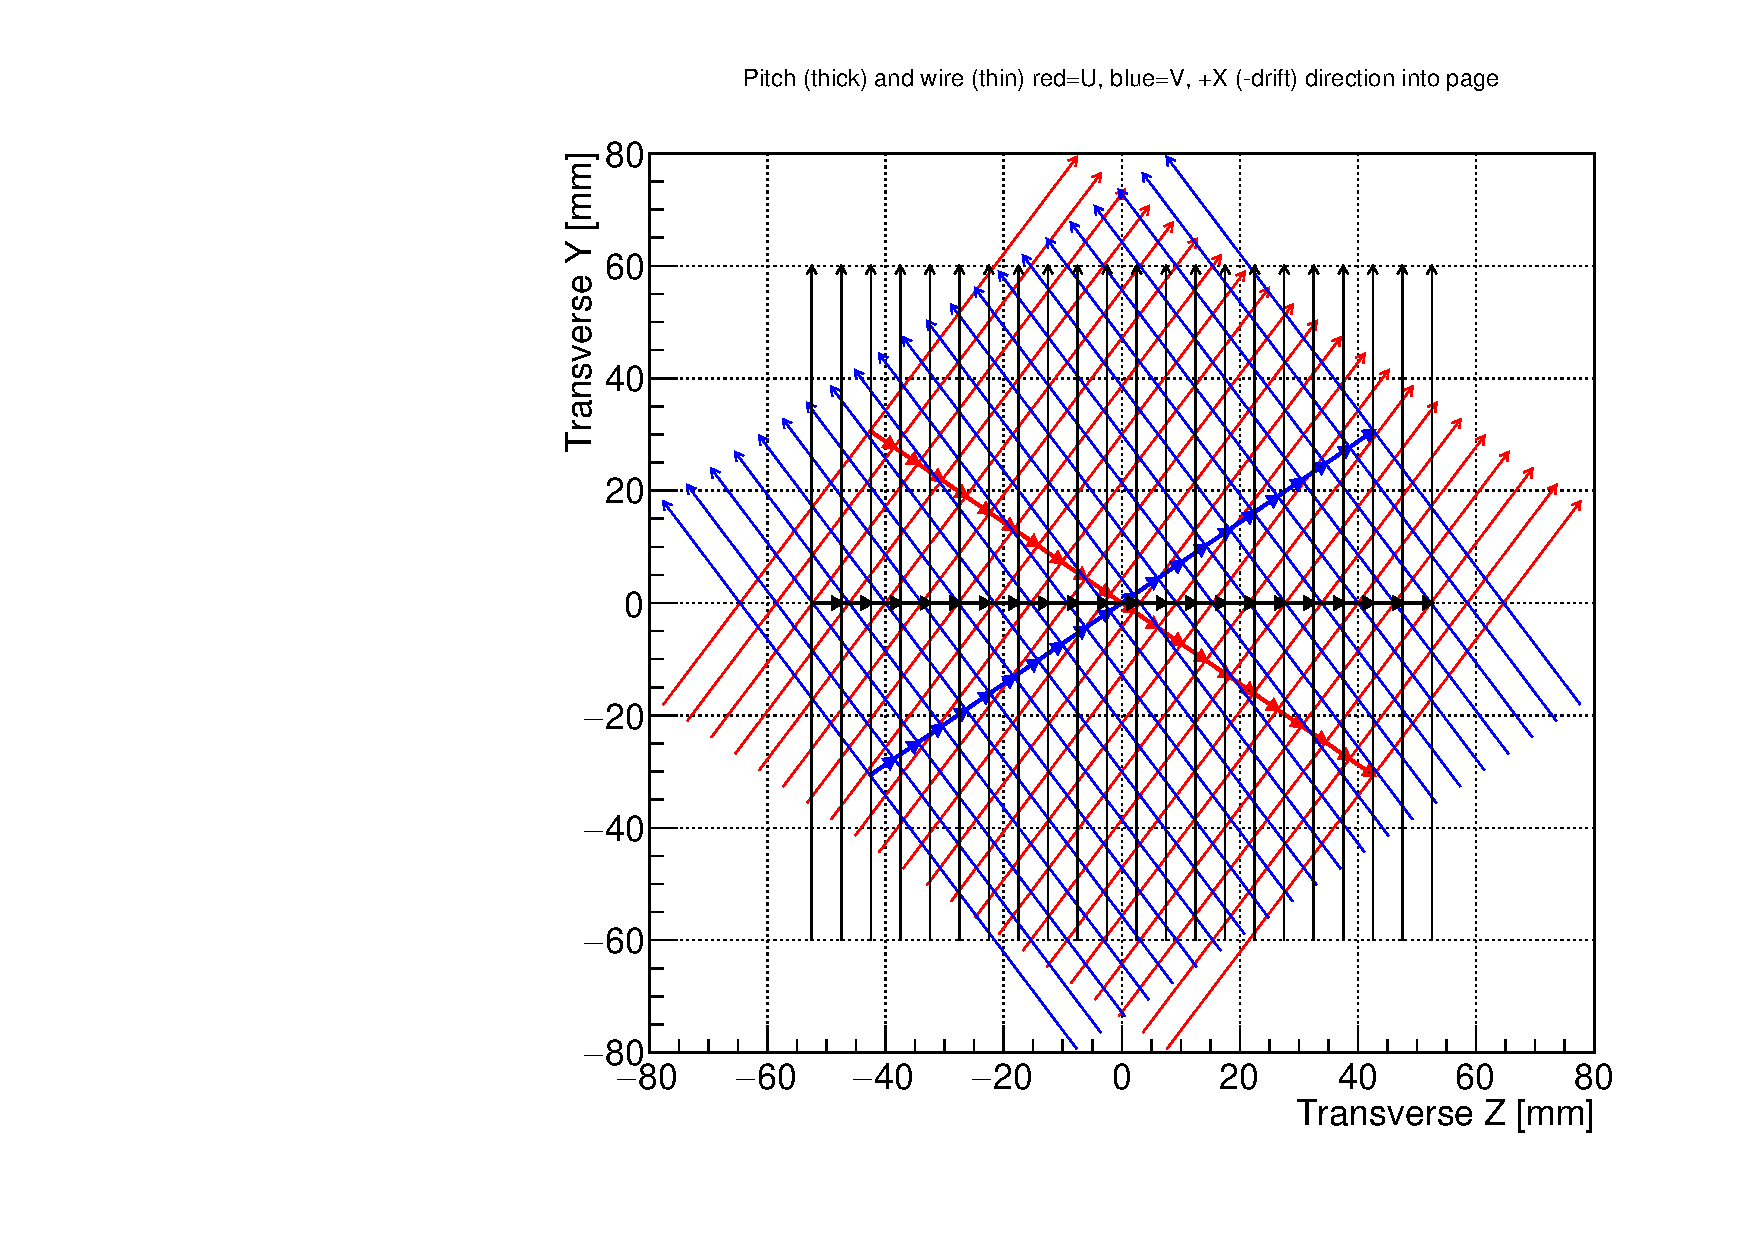
\includegraphics[height=9cm]{test_pimpos_draw.pdf}

      $-z_w \longrightarrow 0 \longrightarrow +z_w$
    \end{center}
  \end{minipage}
  \begin{minipage}[t][10cm][t]{0.39\textwidth}
    \begin{center}
      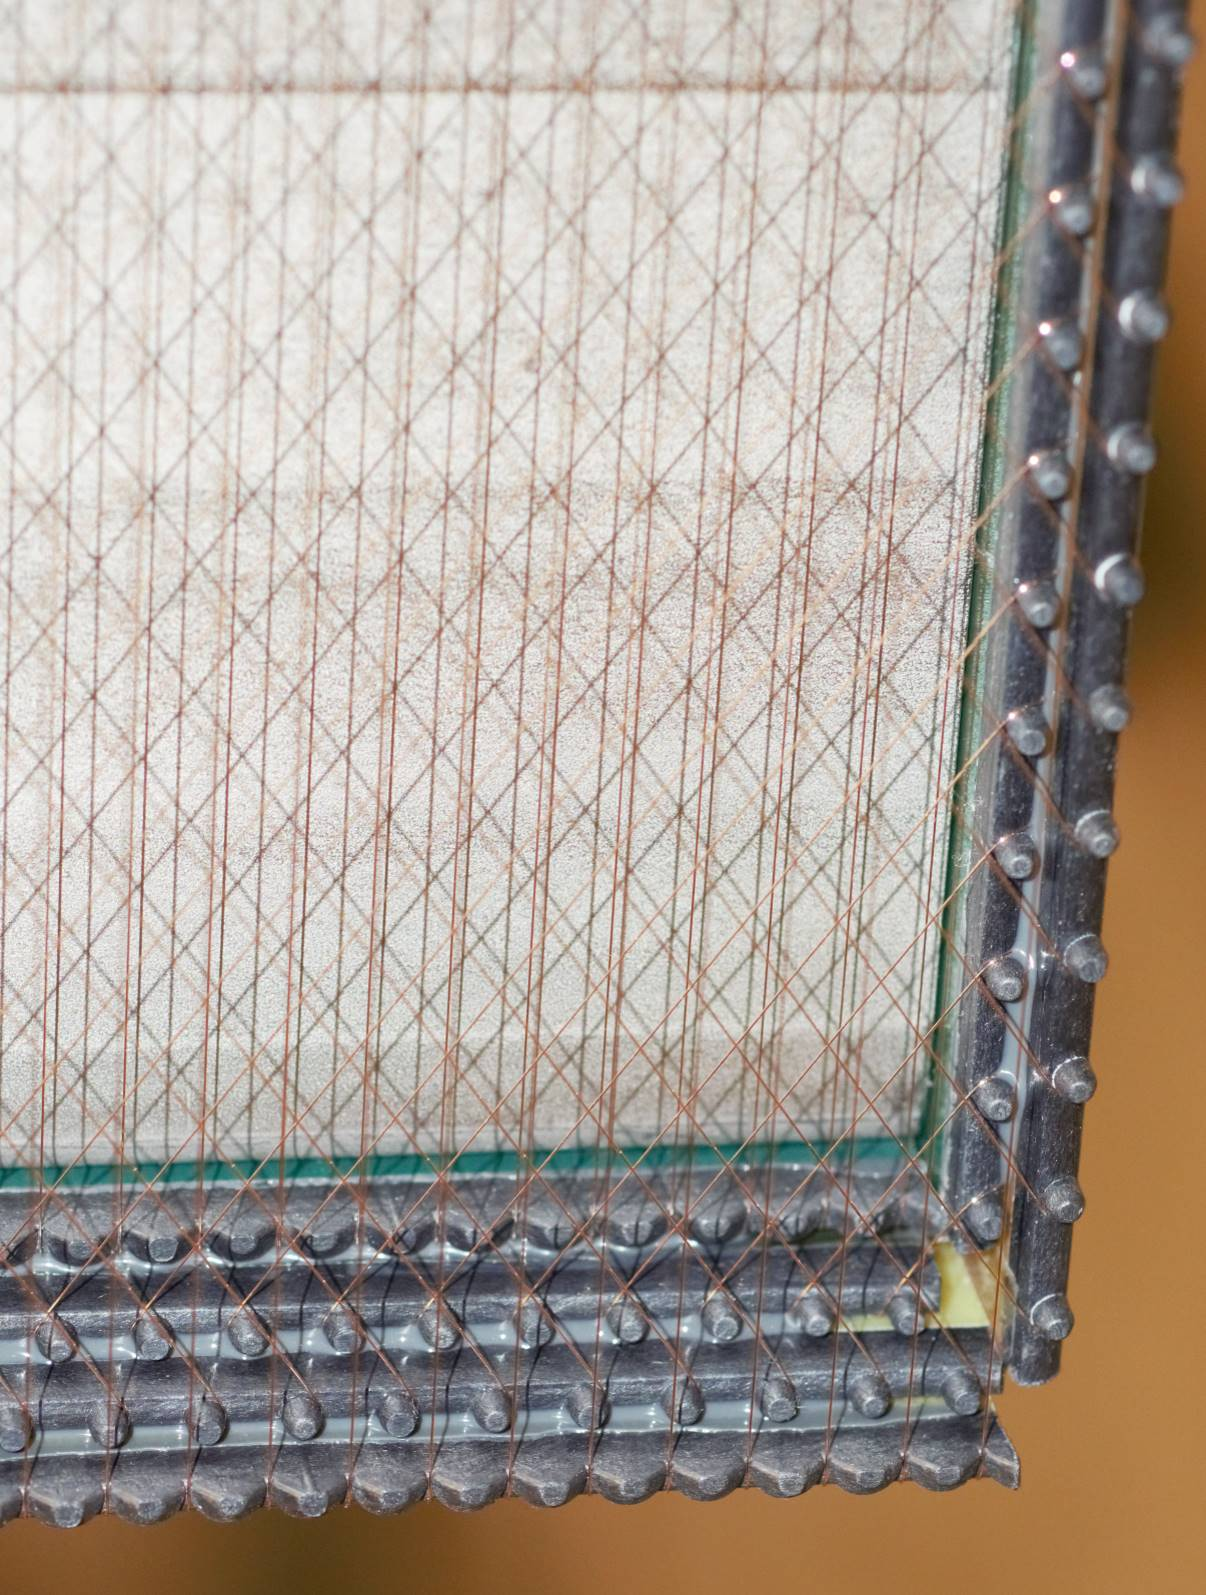
\includegraphics[height=9cm]{others/APA1-wire-photo-bo-yu.jpg}
      
      $+z_w \longleftarrow 0 \longleftarrow -z_w$
    \end{center}
  \end{minipage}

  \caption{Illustration of the three wire coordinate systems relative
    to their parent chamber coordinate system, limited to the
    transverse plane and a photo of the bottom right corner of an APA
    (Bo Yu).  For each plane \textcolor{red}{U in red},
    \textcolor{blue}{V in blue} and \textbf{W in black}, the thin
    arrows are along the wire ($y_w$) direction, the thick arrows are
    along the pitch ($z_w$) direction. The axes of the plot represent
    the $y_c$ and $z_c$ axes.  Into the page are the common $x_c$ and
    the three $x_w$, one for each plane.  The photo shows grid, U, V and W
    wire planes.  Note that the illustration and the photo are viewed
    from different sides.  In the photo the $z_w$ axis points to the
    left.  The U/V wires in each representation are equivalent.}
  \label{fig:coords}
\end{figure}

\section{Connections}

The type of connections defined in the schema graph shown in
Fig.~\ref{fig:schema} require local numbering conventions so that the
children may take some order inside their parent and that this
ordering be meaningfully mapped to physical connections in the
protoDUNE design.  Internally, the graph uses \textbf{zero-based
  indices} but the numbers presented here are expressed as
\textbf{one-based counts}.

The following subsections consider different paths within connection
graph and illustrate various features.  It can be helpful to refer
back to Fig.~\ref{fig:schema} to provide orientation.

\subsection{Detector-APA}

The single-phase protoDUNE detector has six APAs.  The local numbering
convention used here follows the one created by the installation group
and illustrated in Table~\ref{tab:tpc}.  It is worth noting that it
\textit{rasters} the count whereas, as shown below, most other number
assignments observe $180^\circ$ wrapped rotation symmetry.  The
numbering at this scale can be relatively easily extended to the full
DUNE FD with the exception that this detector module will contain some
APA that have central drift volumes on both faces.


\begin{table}[htp]
  
  \centering
  \begin{tabular}[h]{|c|c|c|}
    \hline
    \hline
    \hline
    APA-6 & APA-5 & APA-4\\
    \hline
    \multicolumn{3}{|c|}{}\\
    \multicolumn{3}{|c|}{central drift volume}\\
    \multicolumn{3}{|c|}{}\\
    \hline
    \hline
    \hline
    \multicolumn{3}{|c|}{}\\
    \multicolumn{3}{|c|}{central drift volume}\\
    \multicolumn{3}{|c|}{}\\
    \hline
    APA-3 & APA-2 & APA-1\\
    \hline
    \hline
    \hline
  \end{tabular}

  beam $\longrightarrow$

  \caption{Detector-APA connection indices as viewed looking down on
    the detector and following the order of the installation group
    numbering.}
  \label{tab:tpc}

\end{table}


\subsection{APA-Face-Board}

Each APA has two faces of wires and electronics.  Both are required
for meaningful data.  The first face is taken as being toward a
central drift volume and is identified with index zero.  The other is
toward the nearby cryostat wall and identified with index one.  This
is illustrated for all APAs in Table.~\ref{tab:anodeface}.

\begin{table}[htp]
  \centering
  \begin{tabular}[h]{|c|c|c|}
    \hline
    \hline
    \multicolumn{3}{|c|}{croyostat}\\
    \hline
    face-2 & face-2 & face-2 \\
    \hline
    (frame) & (frame) & (frame) \\
    \hline
    face-1 & face-1 & face-1 \\
    \hline
    \multicolumn{3}{|c|}{}\\
    \multicolumn{3}{|c|}{central drift volume}\\
    \multicolumn{3}{|c|}{}\\
    \hline
    \hline
    \hline
    \multicolumn{3}{|c|}{}\\
    \multicolumn{3}{|c|}{central drift volume}\\
    \multicolumn{3}{|c|}{}\\
    \hline
    face-1 & face-1 & face-1 \\
    \hline
    (frame) & (frame) & (frame) \\
    \hline
    face-2 & face-2 & face-2 \\
    \hline
    \multicolumn{3}{|c|}{cryostat}\\
    \hline
    \hline
    \multicolumn{3}{c}{beam $\longrightarrow$} \\    

  \end{tabular}
  \caption{Anode-face connection indices.  Regardless of the APA, face-1 is toward the central drift volume.}
  \label{tab:anodeface}
\end{table}

Each face contains ten cold electronics boxes holding one cold
front-end electronics board and equivalently for the purposes of this
note, a wire board.  Theses boxes are counted 1-10 in left-to-right
order when looking at the face that contains them and as shown in
Fig.~\ref{fig:wibflange}.  The blue and red dots labeled b1-b10
represent boxes 1-10 on face-1 and those labeled b11-b20 are boxes 1-10
on face-2.

\begin{figure}[h]
  \centering
  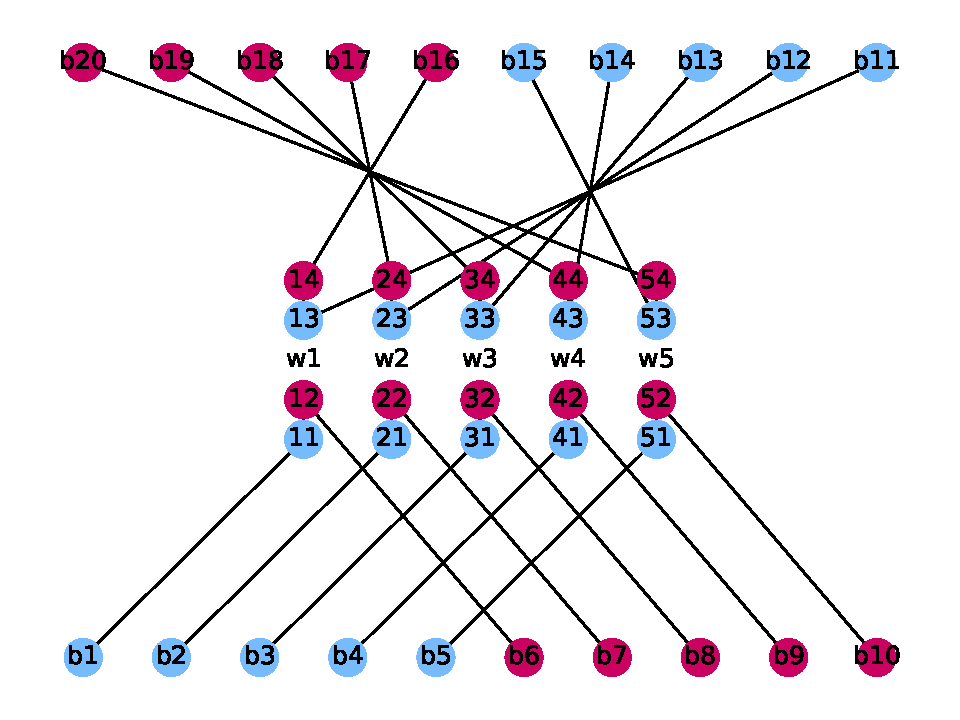
\includegraphics[height=7cm]{test_plot_wib.pdf}%
  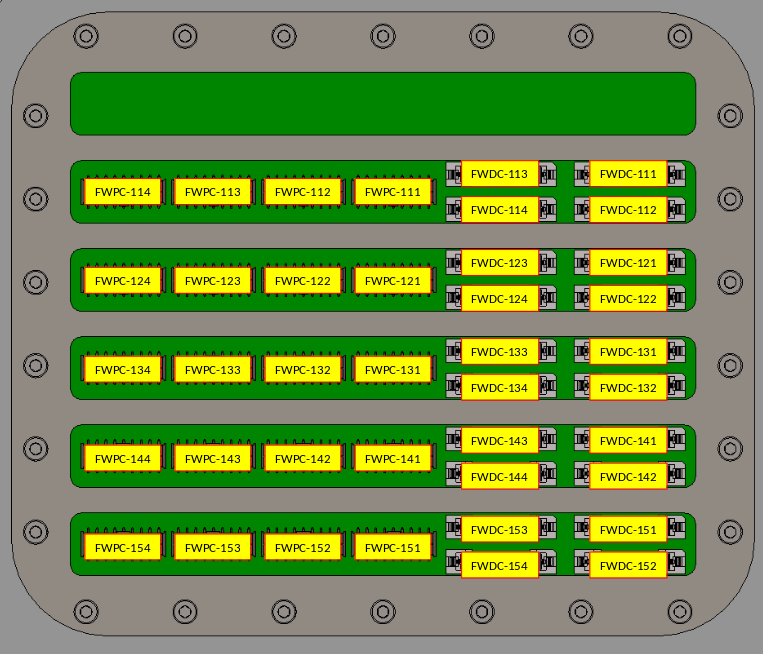
\includegraphics[height=7cm]{others/manhong-ce-mapping-wib.png}

  \caption{\textbf{On the left}, logical connections between boards in
    cold electronics boxes lined up on either face of an APA and the
    warm interface board connectors.  The filled circles on the left
    marked b1-b10 represent CE boxes on APA (front) face-1 and b11-b20
    on (back) face-2.  The points marked w1-w5 represent the five WIBs
    with each of their connectors shown above and below and numbered
    to match the data connectors on the warm interface flange.
    \textbf{On the right}, a drawing from Manhong Zhao showing
    front-end power (FWPC) and data (FWC) connectors through the warm
    interface flange.  The three digit numbers encode a triple of
    numbers for: APA, WIB/slot and connector.}
  \label{fig:wibflange}
\end{figure}

\subsection{APA-WIB-Board}

Each APA has a single warm electronics crate with five slots, each
holding one WIB.  Each WIB has four connectors attaching a data cable
from one board.  Power cables are not considered here but are expected
to follow the data cable assignments shown (and are depicted in Fig.~\ref{fig:wibflange}).

Table~\ref{tab:femb-wib-1} shows the WIB-board connectivity map for a
column of APAs.  Note the rotational symmetry between the pair of APAs
arises simply from keeping
all APAs identical.  Also note the ``WIB-major'' ordering of the two
dimensional array of: $[4\ \mbox{connectors} \times 5\ \mbox{WIBs}]$.
Figure~\ref{fig:wibflange} shows a graphical visualization of their
connections as well as the physical layout of the data connectors on
the warm interface flange.

\begin{table}[htp]
  \centering
  \begin{tabular}[h]{|c|c|c|c|c|c|c|c|c|c|}
    \hline
    \multicolumn{10}{|c|}{Cryostat wall} \\
    \hline
    WIB 5 & WIB 4 & WIB 3 & WIB 2 & WIB 1 & WIB 5 & WIB 4 & WIB 3 & WIB 2 & WIB 1 \\
    \multicolumn{5}{|c|}{WIB connector 4} & \multicolumn{5}{c|}{WIB connector 3} \\
    \hline
    \multicolumn{10}{|c|}{APA frame (APA-6, APA-5 or APA-4)} \\
    \hline
    \multicolumn{5}{|c|}{WIB connector 1} & \multicolumn{5}{c|}{WIB connector 2} \\
    WIB 1 & WIB 2 & WIB 3 & WIB 4 & WIB 5 & WIB 1 & WIB 2 & WIB 3 & WIB 4 & WIB 5\\
    \hline
    \multicolumn{10}{|c|}{} \\
    \multicolumn{10}{|c|}{central drift volume} \\
    \multicolumn{10}{|c|}{} \\
    \hline
    \hline
    \hline
    \multicolumn{10}{|c|}{} \\
    \multicolumn{10}{|c|}{central drift volume} \\
    \multicolumn{10}{|c|}{} \\
    \hline
    WIB 5 & WIB 4 & WIB 3 & WIB 2 & WIB 1 & WIB 5 & WIB 4 & WIB 3 & WIB 2 & WIB 1\\
    \multicolumn{5}{|c|}{WIB connector 2} & \multicolumn{5}{c|}{WIB connector 1} \\
    \hline
    \multicolumn{10}{|c|}{APA frame (APA-3, APA-2 or APA-1)} \\
    \hline
    \multicolumn{5}{|c|}{WIB connector 3} & \multicolumn{5}{c|}{WIB connector 4} \\
    WIB 1 & WIB 2 & WIB 3 & WIB 4 & WIB 5 & WIB 1 & WIB 2 & WIB 3 & WIB 4 & WIB 5\\
    \hline
    \multicolumn{10}{|c|}{Cryostat wall} \\
    \hline


    \multicolumn{10}{c}{beam $\longrightarrow$} \\    
  \end{tabular}
  \caption{FEMB-WIB connectivity for one column of APAs.  The mapping
    is performed in ``WIB-major'' order which wraps around the APA
    frame advancing the WIB connector number once for each half frame.
    Because the APAs are constructed identically, after installation a
    pair of APAs in the same column exhibit $180^\circ$
    rotational symmetry so that the low numbered connectors
    (1 and 2) in every crate will service the conductors attached on the face
    toward the central drift volume and the high numbered (3 and 4)
    connectors will service the conductors attached to the face toward the
    cryostat wall.  Each column of APAs exhibit simple translational
    symmetry with their neighbors.}
  \label{tab:femb-wib-1}
\end{table}

This WIB-major layout allows for simple iterations on WIB connector
and WIB slot as part of iterating on the line of conductors attachment
spots on a face.  A second layout based on $2 \times 2 \times 5$
blocks of boards was considered.  Its connector-major is maybe more
intuitive but mapping that pattern to the boards and their wires leads
to somewhat higher complexity and  more convoluted iterations.


\subsection{Board-Chip-Channel-Conductor}

Each board has eight chips and each chip has 16 channels each of which
connects to one conductor.  The conductor is also identified with a
row and a spot on a wire board.  Each row is identified with one plane
of a face and the spots in a row are identified with a sequence of
neighboring wires.  The complex shuffle between the pair (chip,
channel) and the pair (row, spot) is summarized by the matrix in
Table~\ref{tab:wirechmap}.  The connections between a board of chips
and their channels to the lines of spots in each plane where
conductors attach are visualized in Figure~\ref{fig:boardchip}.  

\begin{table}[htp]
  \centering

  % generated by chmap.py using files:
% others/shanshan/ProtoDUNE_APA_Wire_Mapping_091917_v3-J1.csv
% others/shanshan/ProtoDUNE_APA_Wire_Mapping_091917_v3-J2.csv
\begin{tabular}{r|rrrrrrrr}
\hline
ASIC:&1&2&3&4&5&6&7&8\\
\hline
ch00 & \textcolor{red}{u19} & \textcolor{red}{u09} & \textcolor{black}{w14} & \textcolor{black}{w02} & \textcolor{red}{u29} & \textcolor{red}{u39} & \textcolor{black}{w26} & \textcolor{black}{w38}\\
ch01 & \textcolor{red}{u17} & \textcolor{red}{u07} & \textcolor{black}{w16} & \textcolor{black}{w04} & \textcolor{red}{u27} & \textcolor{red}{u37} & \textcolor{black}{w28} & \textcolor{black}{w40}\\
ch02 & \textcolor{red}{u15} & \textcolor{red}{u05} & \textcolor{black}{w18} & \textcolor{black}{w06} & \textcolor{red}{u25} & \textcolor{red}{u35} & \textcolor{black}{w30} & \textcolor{black}{w42}\\
ch03 & \textcolor{red}{u13} & \textcolor{red}{u03} & \textcolor{black}{w20} & \textcolor{black}{w08} & \textcolor{red}{u23} & \textcolor{red}{u33} & \textcolor{black}{w32} & \textcolor{black}{w44}\\
ch04 & \textcolor{red}{u11} & \textcolor{red}{u01} & \textcolor{black}{w22} & \textcolor{black}{w10} & \textcolor{red}{u21} & \textcolor{red}{u31} & \textcolor{black}{w34} & \textcolor{black}{w46}\\
ch05 & \textcolor{blue}{v19} & \textcolor{blue}{v09} & \textcolor{black}{w24} & \textcolor{black}{w12} & \textcolor{blue}{v29} & \textcolor{blue}{v39} & \textcolor{black}{w36} & \textcolor{black}{w48}\\
ch06 & \textcolor{blue}{v17} & \textcolor{blue}{v07} & \textcolor{blue}{v12} & \textcolor{blue}{v02} & \textcolor{blue}{v27} & \textcolor{blue}{v37} & \textcolor{blue}{v22} & \textcolor{blue}{v32}\\
ch07 & \textcolor{blue}{v15} & \textcolor{blue}{v05} & \textcolor{blue}{v14} & \textcolor{blue}{v04} & \textcolor{blue}{v25} & \textcolor{blue}{v35} & \textcolor{blue}{v24} & \textcolor{blue}{v34}\\
ch08 & \textcolor{blue}{v13} & \textcolor{blue}{v03} & \textcolor{blue}{v16} & \textcolor{blue}{v06} & \textcolor{blue}{v23} & \textcolor{blue}{v33} & \textcolor{blue}{v26} & \textcolor{blue}{v36}\\
ch09 & \textcolor{blue}{v11} & \textcolor{blue}{v01} & \textcolor{blue}{v18} & \textcolor{blue}{v08} & \textcolor{blue}{v21} & \textcolor{blue}{v31} & \textcolor{blue}{v28} & \textcolor{blue}{v38}\\
ch10 & \textcolor{black}{w23} & \textcolor{black}{w11} & \textcolor{blue}{v20} & \textcolor{blue}{v10} & \textcolor{black}{w35} & \textcolor{black}{w47} & \textcolor{blue}{v30} & \textcolor{blue}{v40}\\
ch11 & \textcolor{black}{w21} & \textcolor{black}{w09} & \textcolor{red}{u12} & \textcolor{red}{u02} & \textcolor{black}{w33} & \textcolor{black}{w45} & \textcolor{red}{u22} & \textcolor{red}{u32}\\
ch12 & \textcolor{black}{w19} & \textcolor{black}{w07} & \textcolor{red}{u14} & \textcolor{red}{u04} & \textcolor{black}{w31} & \textcolor{black}{w43} & \textcolor{red}{u24} & \textcolor{red}{u34}\\
ch13 & \textcolor{black}{w17} & \textcolor{black}{w05} & \textcolor{red}{u16} & \textcolor{red}{u06} & \textcolor{black}{w29} & \textcolor{black}{w41} & \textcolor{red}{u26} & \textcolor{red}{u36}\\
ch14 & \textcolor{black}{w15} & \textcolor{black}{w03} & \textcolor{red}{u18} & \textcolor{red}{u08} & \textcolor{black}{w27} & \textcolor{black}{w39} & \textcolor{red}{u28} & \textcolor{red}{u38}\\
ch15 & \textcolor{black}{w13} & \textcolor{black}{w01} & \textcolor{red}{u20} & \textcolor{red}{u10} & \textcolor{black}{w25} & \textcolor{black}{w37} & \textcolor{red}{u30} & \textcolor{red}{u40}\\
\hline
\end{tabular}


  \caption{The per-board connections between a chip (columns) and its
    channel (rows, one-based count) and the local numbering the row
    and spot for a conductor connection.  The row is identified by a
    plane letter (``u'', ``v'' or ``w'') and the spot is a numbered
    count starting from one (not zero).  Counts are
    \textcolor{red}{1-40 for U plane and marked in red},
    \textcolor{blue}{1-40 for V plane and marked in blue} and
    \textbf{1-48 for W plane and marked in black}.  This pattern is
    applied for each board on each face of an APA.}
  \label{tab:wirechmap}
\end{table}


\begin{figure}[h]
  \centering
  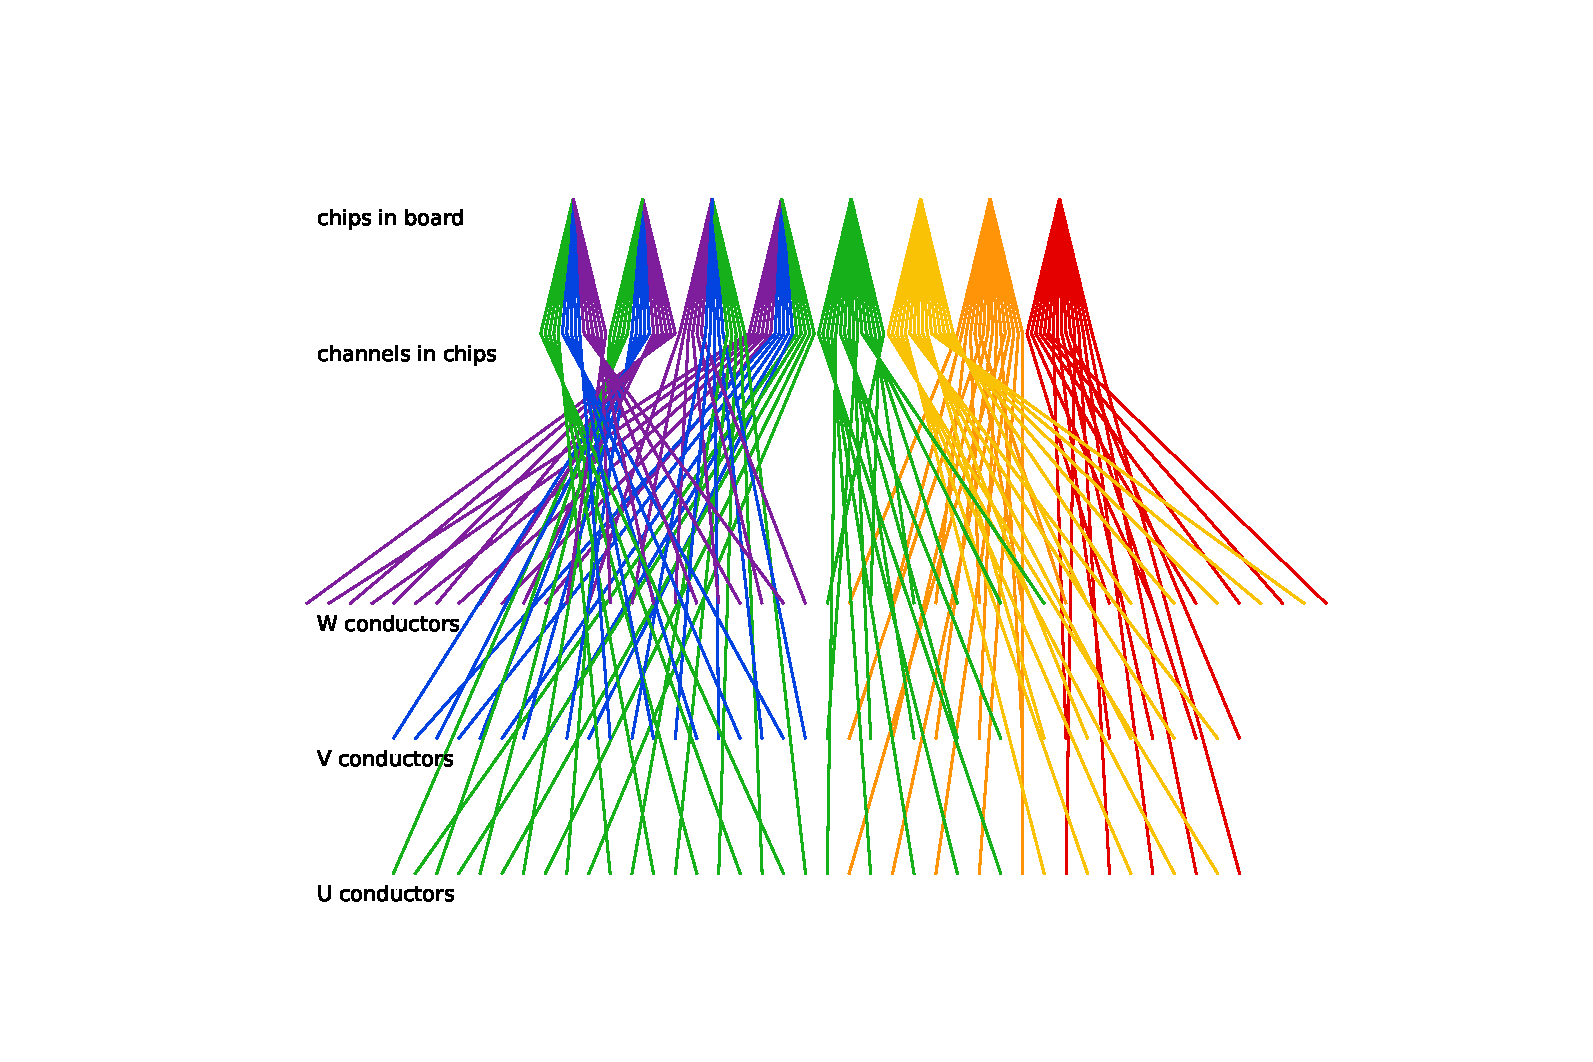
\includegraphics[width=\textwidth]{test_plot_board_chip.pdf}
  \caption{Visualization of the connectivity between the channels of the eight chips on one board and the conductors attaching at a given spot in a row on the associated wireboard.  The channels of the first four chips are colored according to the wire board row (plane) they service.  The channels from the last four chips are colored by their chip number.}
  \label{fig:boardchip}
\end{figure}


\subsection{Conductor-Wire}

Figure~\ref{fig:wires} visualizes a sampling of wire segments separated
by the planes in an APA face where they reside.  They are drawn consistent with
Fig.~\ref{fig:coords} and in particular with the same caution that one
is viewing the wires looking in the $+x$ direction which is counter to the nominal
electron drift (ie, ``behind'' the wires).  In all cases the index of a wire in its plane is
counted starting at the wire with its center at the most negative Z detector
location which also corresponds to the most negative
pitch location for that plane.  For the U plane, this first wire is at the top of the APA, for
the V plane it is at the bottom.  Note, this convention has the
wire-in-plane index run generally counter to the direction that a face's
boards or a board's conductor spots are numbered.  


\begin{figure}[htp]
  \centering
  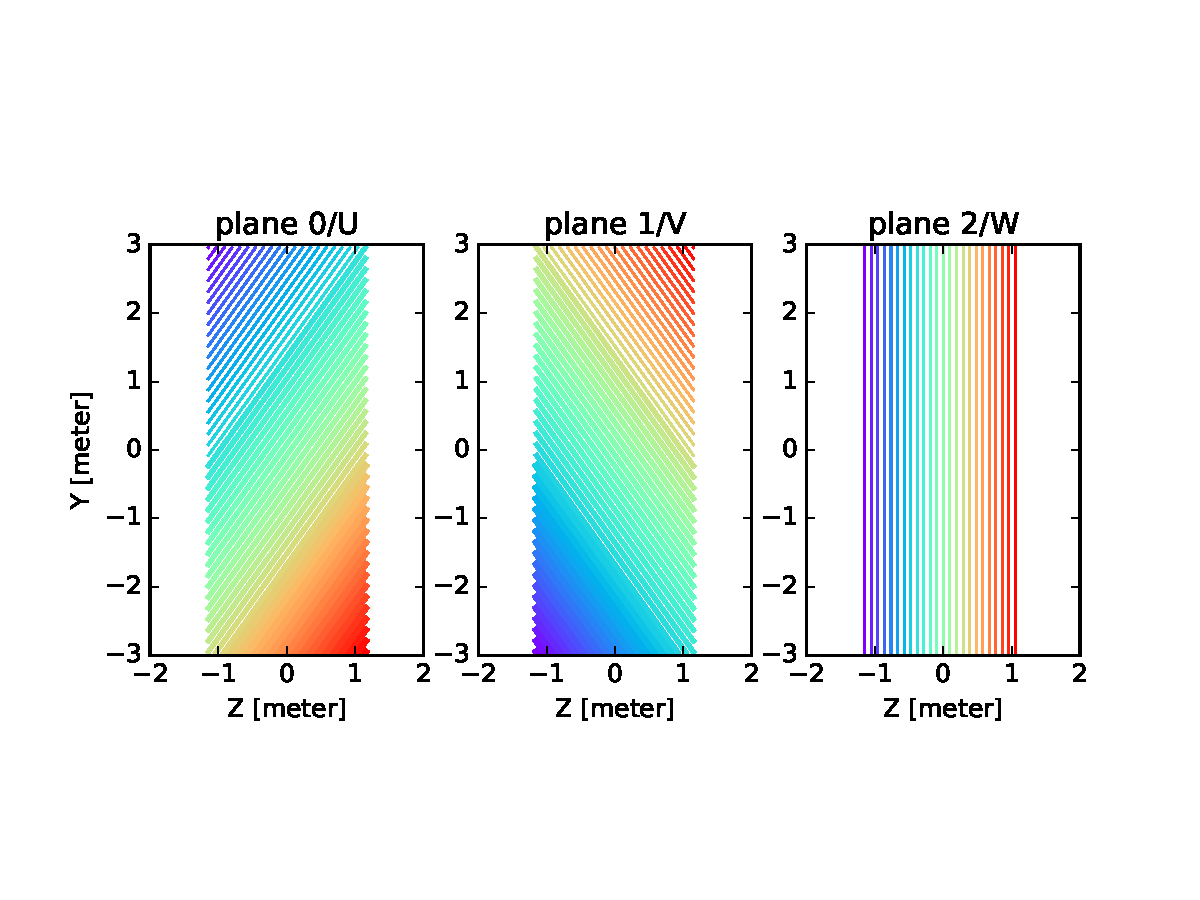
\includegraphics[width=\textwidth,clip,trim=0 3cm 0 3cm]{wires-20.pdf}
  \caption{The wire (segments) for each wire plane on one face of one APA for protoDUNE.  Increasing line width indicates increasing \textbf{segment number} $\in$ (0, 1 or 2).  The color indicates increasing \textbf{wire index} from blue to red.  Only one of every twenty wires are shown. The Y coordinate points opposite of gravity.  The unlabeled X coordinate runs into the page and is counter to the drift direction.  Z follows from the right-hand-rule.}
  \label{fig:wires}
\end{figure}


\subsection{Board-Chip-Conductor-Wire}

Each board services 128 conductors.  These conductors may wrap around
zero, once or twice depending on which plane they are in and where the
conductors enter the plane.  Figure~\ref{fig:board} visualizes the
location of the wires from each of the ten boards on one face.  Take
note that every other conductor in a given plane is serviced by a
different chip as governed by the matrix in Table~\ref{tab:wirechmap}.

\begin{figure}[h]
  \centering

  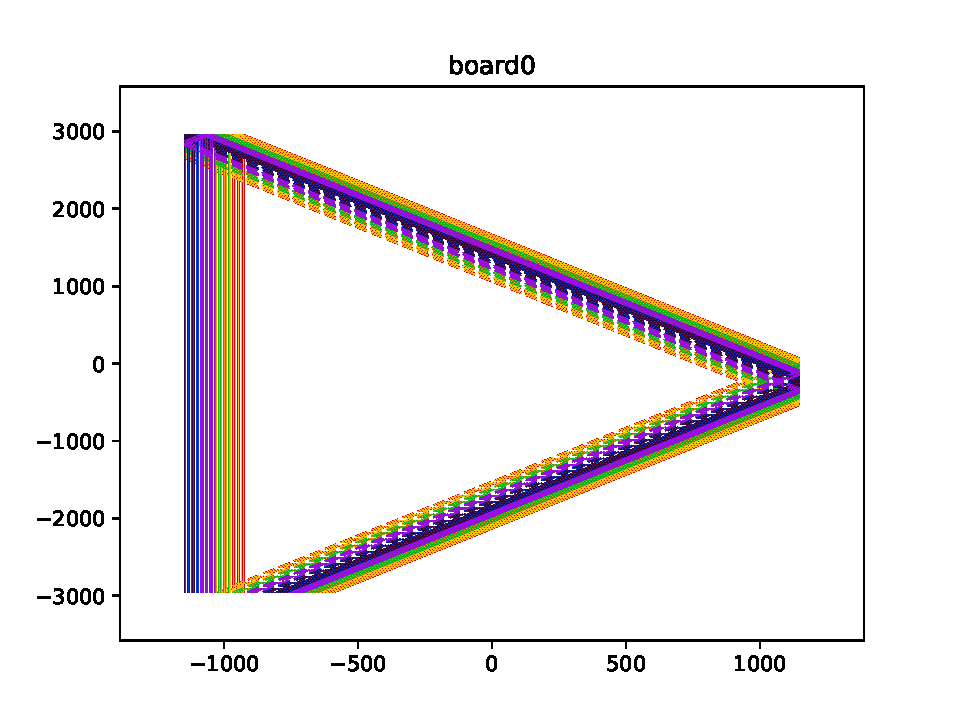
\includegraphics[height=7cm,page=1,clip, trim=4cm 0 5cm 0]{test_plot_board.pdf}%
  \includegraphics[height=7cm,page=2,clip, trim=5cm 0 5cm 0]{test_plot_board.pdf}%
  \includegraphics[height=7cm,page=3,clip, trim=5cm 0 5cm 0]{test_plot_board.pdf}%
  \includegraphics[height=7cm,page=4,clip, trim=5cm 0 5cm 0]{test_plot_board.pdf}%
  \includegraphics[height=7cm,page=5,clip, trim=5cm 0 5cm 0]{test_plot_board.pdf}%

  \includegraphics[height=7cm,page=6,clip, trim=4cm 0 5cm 0]{test_plot_board.pdf}%
  \includegraphics[height=7cm,page=7,clip, trim=5cm 0 5cm 0]{test_plot_board.pdf}%
  \includegraphics[height=7cm,page=8,clip, trim=5cm 0 5cm 0]{test_plot_board.pdf}%
  \includegraphics[height=7cm,page=9,clip, trim=5cm 0 5cm 0]{test_plot_board.pdf}%
  \includegraphics[height=7cm,page=10,clip, trim=5cm 0 5cm 0]{test_plot_board.pdf}%
  

  \includegraphics[height=5cm,page=3,clip,trim=7.1cm 9.4cm 8.1cm 2.25cm]{test_plot_board.pdf}%
  \includegraphics[height=5cm,page=3,clip,trim=6.8cm 8.6cm 9cm 3.1cm]{test_plot_board.pdf}

  \caption{The location of wires, in chamber coordinates ($z_c,y_c$)
    for the ten boards on one face.  Wires are colored by the chip to
    which their conductor is connected.  Wires that are wrapped around
    to the other face are dashed.  Note: depending on the technology
    used to view these image, many fine details may be obscured.  The
    final row of two plots show zoomed regions of the top left corner
    of the third board (``Board 3'').  The left figure shows wires
    from each three planes from their attachment points at the top of
    the APA.  The right figure shows U wires as they wrap around the
    frame and continue on as U wires on the opposite face.}
  \label{fig:board}
\end{figure}


\section{Global Numbering}

The numbers described so far are local defined local to each type of
connection.  As the same type of connection takes part in some larger
scale, these local numbers are reused.  For example, the same 16
channel indices are used for all chips.  This local numbering requires
adopting some convention in order to associate the connections to the
real-world.  The resulting directed, cyclic graph representation is
not convenient for typical linear programming paradigms.  So, it is
useful to flatten the graph to some ordered sequence containing
identifiers that are unique to some context, small and in some cases
may be used as dense indices.  This requires asserting some stronger
and broader and typically ad-hoc but well intentioned convention.

For example, LArSoft requires an exhaustive list of every wire segment
across the entire detector and it assumes ``channel'' numbers which
are conceptually more similar to the conductor attachment spots on the
wire boards.  In another, the Wire-Cell Toolkit simulation is
optimized by addressing wires in their plane as a regular array
ordered by their pitch location.

Such special case conventions can be accommodated by writing a
function that traverses the full connectivity graph and applies some
transformation to its minimal numbering convention in order to produce
identifiers in some other desired scheme.

\subsection{The Channel Numbering Problem}

It is of course very typical to speak of ``the channel number'' to
identify some measured data with either a portion of the electronics
or a portion of the physical detector.  This number ideally has the
characteristics that it is globally unique in the detector, it is
monotonically increasing without gaps and that various ranges of the
sequence map in some simple way to either groups of electronics
components or to contiguous portions of the detector or both.  To the
extent that these desired characteristics can be satisfied, people may
develop the ability to mentally map data plotted vs ``channel'' number
to electrical or physical space and thus better understand the content
of plots and figures.

With protoDUNE APAs, due to the per-board connectivity shown in the
matrix of Table~\ref{tab:wirechmap}, all these ideals are largely
impossible to achieve fully.  This difficulty can also be seen by examining
the wires colored by their chip in Fig.~\ref{fig:board}.  There is no
single, natural ordering of ``channels'' which is coherent with both
electronic and physical spaces.

Even simple coherency with physical space is impossible due to the
wrapped wires.  However, within one plane of one face of one APA there
is one natural physical ordering of the line of ``spots'' where the
conductors attach to the wire boards.  There are 400 U,
400 V and 480 W spots each in their own line in their face.  A
``channel'' number based on this ordering provides a partially
coherent enumeration of some contiguous regions of the detector.  It
fails, of course, as soon as one considers regions where wrapping
occurs.  And, as shown in Fig.~\ref{fig:boardchip}, it does not lend
to any simple mapping into electronics space.

Finally, real data from the DAQ will of course not include spot
identifiers but rather carry crate address, WIB slot and connector
numbers which identify the data stream as coming from one FEMB.  Which
FEMB relies on proper cabling following Table~\ref{tab:femb-wib-1}.
Within those streams will be vectors of per-tick samples that map
implicitly to a fixed layout of chips and their channels.  Mapping
this vector to the axes of the matrix in Table~\ref{tab:wirechmap} is
not yet specified but once done one can form a composite number with
suitable combinations of the local connection numbers.  This composite
number can be constructed in such a way (see below) as to give some
immediate understanding of the electronics component it refers.
However, it will not be monotonic in any simple ordering and will,
again, have no simple mapping to physical space.

So, it must be accepted that there is no single best choice for a
global channel numbering scheme.  Instead, multiple schemes must be
expected to be used in actual day-to-day practice.  The following
sections offer suggestions for how to construct global channel numbers
in ways that cover two important contexts.

\subsection{Global Electronics Channel Number}

Referring to Fig.~\ref{fig:schema} it is clear that there are two
simple ways to refer to an electronics channel.  The first is a
\textit{data-centric} view and consists of using the identifiers that
will exist in the raw data.  A channel may be addressed by the
following 5-tuple where \texttt{slot\#} counts the WIB and
\texttt{address\#} is used instead of the word ``channel'' to avoid
ambiguity.

\begin{description}
\item[\texttt{apa\#}] 1-6 (1-150 for DUNE FD)
\item[\texttt{connector\#}] 1-5
\item[\texttt{slot\#}] 1-4
\item[\texttt{chip\#}] 1-8
\item[\texttt{address\#}] 01-16
\end{description}

\noindent 
Given this tuple, it is recommended to create a decimal-composite
\textit{global electronics channel number} by padding them by factors
of ten and with the address padded by an extra factor of 10.  Using
the first letter of their label in the order above it would give
numbers like: ``\texttt{ACSCAA}''.  Note, one-based counts are
explicitly used here to avoid creating any special ``0'' channel and
to preserve padding.
While these numbers present a sparse sequence, they do allow some
natural ordering.  A human can apply a decimal mask to easily recover
the individual component numbers.

The second simple way to refer to an electronics channel is
\textit{position-centric} and is formed by traveling through the graph of
Fig.~\ref{fig:schema} via a face instead of a WIB.  Face and box
numbers will not appear in the raw data but given the \textit{global
electronics channel number} derived as above, and knowledge of the
simple pattern of Table~\ref{tab:femb-wib-1}, it is relatively easy to
understand in what face and box the channel resides.

\subsection{Global Conductor Channel Number}

As already mentioned, the most natural channel numbering scheme
possible which has at least some coherency with physical space while
still retaining some coherency with electronics space is based on the
line of conductor attachment points at the top of an APA frame.  Given
the wire wrapping it would be most natural to construct a global conductor
channel number composed of these components:

\begin{description}
\item[\texttt{apa\#}] 1-6 (1-150 for DUNE FD)
\item[\texttt{plane\#}] 1-3
\item[\texttt{spot\#}] U:1-800, V:1-800, W:1-960
\end{description}

\noindent Note these account for both faces of an APA.
It is recommended to compose them in a similar manner as the global
electronics channel number producing ``\texttt{APSSS}''.
Table~\ref{tab:gccn} shows how these map to physical locations.

\begin{table}[htp]
  
  \centering
  \begin{tabular}[h]{|c|c|c|}
    \hline
    61800 -- 61401 & 51800 -- 53401 & 41800 -- 43401\\
    62800 -- 62401 & 52800 -- 53401 & 42800 -- 43401\\
    63960 -- 63481 & 53960 -- 53481 & 43960 -- 43481\\
    \hline
    APA-6 frame & APA-5 frame & APA-4 frame \\
    \hline
    63001 -- 63480 & 53001 -- 53480 & 43001 -- 43480\\
    62001 -- 62400 & 52001 -- 53400 & 42001 -- 43400\\
    61001 -- 61400 & 51001 -- 53400 & 41001 -- 43400\\
    \hline
    \multicolumn{3}{|c|}{}\\
    \multicolumn{3}{|c|}{central drift volume}\\
    \multicolumn{3}{|c|}{}\\
    \hline
    \hline
    \hline
    \multicolumn{3}{|c|}{}\\
    \multicolumn{3}{|c|}{central drift volume}\\
    \multicolumn{3}{|c|}{}\\
    \hline
    31400 -- 31001 & 23400 -- 21001 & 13400 -- 11001\\
    32400 -- 32001 & 23400 -- 22001 & 13400 -- 12001\\
    33480 -- 33001 & 23480 -- 23001 & 13480 -- 13001\\
    \hline
    APA-3 frame & APA-2 frame & APA-1 frame \\
    \hline
    33481 -- 33960 & 23481 -- 23960 & 13481 -- 13960\\
    32401 -- 32800 & 23401 -- 22800 & 13401 -- 12800\\
    31401 -- 31800 & 23401 -- 21800 & 13401 -- 11800\\
    \hline
  \end{tabular}

  beam $\longrightarrow$

  \caption{The recommended Global Conductor Channel Numbering scheme.}
  \label{tab:gccn}

\end{table}

The features in favor of this scheme include large contiguous counts
at the wire plane level which will facilitate making plots while
having some granularity at the plane and APA level to assist humans in
visualizing which part of the detector is being referred to.  In all
cases the per-APA/per-plane channel numbers run parallel to their wire
board spots and are related by a simple factor of residual factor of
40 or 48 which assists in mentally drilling down to the board level.
Their low range is always facing the central drift volume which
preserves the $180^\circ$ wrapped rotational symmetry of the six APAs
in the detector, nicely mimicking the rotational symmetry of the wires
in each APA and allowing one retain a simple mnemonic.


\section{Software}

The software used to generate the full connection graph, up to one APA
is available in the
\href{https://github.com/wirecell/wire-cell-python}{wire-cell-python}
package.  This is a pure Python package developed in support of the
C++ Wire-Cell Toolkit (WCT) which provides many features including
state of the art noise filtering and signal processing used by
MicroBooNE as well as a general purpose noise and signal simulation
which has various improvements over prior codes.  The Python package
can be installed and run like any Python package and in particular,
independent from the WCT C++ packages.

Generating the full connection graph requires just a few lines of
code\footnote{It is expected this package will require some refactoring to be made more generic for other detectors.  Future readers beware that this example may fall out of date.}:

\begin{verbatim}
  from wirecell.util.wires import apa
  desc = apa.Description();
  G,P = apa.graph(desc)
\end{verbatim}

The returned value \texttt{G} is a
\href{https://networkx.github.io/}{NetworkX} graph and as such can be
used along with the many graph-theoretic operations provided.  It can be
persisted to various supported formats.  The visualization services of
NetworkX are what produced most of the figures in this note.  The
second returned value \texttt{P} is not explicitly needed but provides
a simple \texttt{namedtuple} allowing easy access to nodes of the
different types in the order in which they were created.

The \texttt{apa.Description} class constructor takes an optional set
of parameters defaulting to \\ \texttt{apa.default\_params}.  These
parameters govern many aspects of the graph generation including such
things as:

\begin{itemize}
\item Wire angles, pitch, plane width, height, various locations.
\item Multiplicity of boards, WIBs, their connectors, chips and channels
\item Chip/channel mapping to conductor row and spot (ie, Table~\ref{tab:wirechmap})
\end{itemize}

Utility functions in \texttt{wirecell.util.wires.graph} are provided
which operate on the graph \texttt{G}.  They include flattening the
graph to lists giving channel-level information including that which
follows the global channel numbering conventions described above.
These utilities will need to be expanded as more client software
requires different formats for the information encoded into the
connection graph.

\section{Summary}

A directed, cyclic graph representation of the connections important
for protoDUNE data is described.  It relies on a minimal local
numbering convention to tie its representation of associations to the
real-world detector design.  It takes no stand on global conventions
but it can be used to generate numbers following their schemes.  An
instance of the full connectivity graph based on nominal design
parameters has been generated and validated with various
visualizations, a portion of which are included in this note.  The
problems with defining a single optimal global channel numbering
scheme were described and two complimentary ones were proposed which
cover the important contexts of raw data analysis and of
reconstruction/simulation.  The software used to produce this graph
and flatten it to produce global channel numbering is described and
made available.  It is expected that further development is needed to
satisfy the requirements of users of the connectivity graph as they
become better understood.

\end{document}

%%% Local Variables:
%%% mode: latex
%%% TeX-master: t
%%% End:
